	\begin{center}
		{
			\vspace*{3in}
			\LARGE
			\textsc{
				Problem Set 1
			}
		}
	\end{center}
	\newpage
	% ===========================
	% PROBLEM 1.1
	% ===========================
	\stepcounter{subsection}
	\subsection*{
		Problem 1.1
	}
	\begin{problem}
		Revisit our lecture on ``relativity without light". 
		In one of the final steps, it was assumed that
		\begin{equation}
			\label{eq:1.1}
		    \frac{A(v)^2-1}{v^2 A(v)^2} = k > 0 
		\end{equation}
		Explore the cases $k = 0$ and $k < 0$. 
		Are these viable options? Why or why not?
	\end{problem}
	\begin{solution_pset}
		\nocite{juan2026}

		From the lecture, discussed in \S 1.4 of \cite{juan2026}, aside from the
		derivation of the constant that naturally arises 
		from fundamental assumptions, $k$.
		\begin{equation}
			\label{eq:k-constant}
		    \frac{A^2 - 1}{v^2 A^2} = k 
		\end{equation}
		we also derived the form of the transformation
		between two frames:\footnote{I used $(t,x)$ here
		instead of the presented coordinates in the lecture, 
		$(x,t)$}
		\begin{equation}
			\label{eq:transform}
		    \bmqty{
		    	t'\\x'
		    } 
			=
			A
			\bmqty{
				1  & -kv \\
				-v & 1
			} 
			\bmqty{
				t\\x
			} 
		\end{equation}
		and the value of $A$ as a function of $v$:
		\begin{equation}
			\label{eq:A-value}
			A(v) =
			\frac{1}{\sqrt{1-kv^2}} 
		\end{equation}
		As well as velocity addition under such transformations
		\begin{equation}
			\label{eq:velocity-addition}
		    w
			=
			\frac{u+v}{1+kuv} 
		\end{equation}
		All of this was under the assumption that $k>0$.
		Let's derive a few relations from this, before actually
		taking on the prescribed conditions.

		For (\ref{eq:A-value}), we see that the radical
		$\sqrt{1-kv^2}$ imposes a restriction on the allowed values
		of $v$. The argument of the square root must remain
		nonnegative:
		\begin{align*}
			1-kv^2 &\geq 0,\\
			kv^2 &\leq 1,\\
			v^2 &\leq \frac{1}{k},\\
			\abs{v} &\leq \frac{1}{\sqrt{k}}.
		\end{align*}
		Thus, for $k>0$, $v$ cannot exceed $1/\sqrt{k}$ in magnitude.
		As $v$ approaches this value, the denominator of $A(v)$
		approaches zero and therefore $A(v)$ grows without bound.
		
		To see what this value implies, we try to add this with the velocity
		addition formula. Let $u = \frac{1}{\sqrt{k}}$
		\begin{align}
		    w
			&=
				\frac{
					\frac{1}{\sqrt{k}} +v
				}{
					1+k\frac{1}{\sqrt{k}}v
				} \notag
				\\
			&=
				\frac{
					\frac{1}{\sqrt{k}} +v
				}{
					1+{\sqrt{k}}v
				} \notag
				\\
			&=
				\frac{
					\frac{1 + v\sqrt{k}}{\sqrt{k}}
				}{
					1+{\sqrt{k}}v
				} \notag
				\\
			&=
				\frac{1}{\sqrt{k}} 
				\frac{
					1+{\sqrt{k}}v
				}{
					1+{\sqrt{k}}v
				} \notag
				\\
			&= 
				\frac{1}{\sqrt{k}} 
		\end{align}
		Therefore, the value $\dfrac{1}{\sqrt{k}}$ is invariant.
		It is a fixed point of the velocity-addion law,
		and identifies the invariant limiting speed associated
		with the transformation.
		Let $\kappa$ be
		\begin{equation}
			\label{eq:kappa}
		    \kappa = \frac{1}{\sqrt k} 
		\end{equation}
		By what we found, $\kappa$ must be an invariant quantity, and thus,
		only depends on $k$, which is itself an arbitrary constant. 
	
		Now, we explore what happens when the prescribed conditions are 
		implemented.
		\begin{enumerate}[(1)]
		    \item $k = 0$

				Notice that as we set $k=0$, (\ref{eq:A-value})
				reduces to
				\begin{equation}
					\label{eq:A-1}
				    A = 1
				\end{equation}
				for all $v$.

				Furthermore, the transformation (\ref{eq:transform}) becomes
				\begin{equation}
					\label{eq:galilean-transform}
				    \bmqty{
				    	t'\\x'
				    } 
					=
					\bmqty{
						1 & 0 \\
						-v & 1
					} 
					\bmqty{
						t\\x
					} 
				\end{equation}
				Additionally, when $k\to 0^+$ the invariant limiting speed $\kappa$ tends to infinity.\footnote{It cannot be approached from $0^-$}

				It is effectively a shearing operation on the $S$ frame. (See fig. \ref{fig:lorentzk0})

				This is precisely the classical Galilean transformations.
				Thus, when we set $k=0$, we recover the Galilean transformation,
				where the invariant speed is pushed to infinity, 
				and there is no finite invariant speed.

				This is a \textbf{valid option}, and is in fact the assumption
				adopted by Newtonian and other classical mechanics theories.

			\item $k < 0$

				If we set $k<0$, then (\ref{eq:A-value}) becomes
				\begin{equation}
					\label{eq:A-transform-k<0}
					A(v) = \frac{1}{\sqrt{1+\abs{k}v^2}} 
				\end{equation}
				The condition that the radicand must be greater than 0 is
				satisfied for all $v$, i.e.,
				\[
					\forall v \in \R, k<0, \quad 1 - k v^2 \geq 0
				\]
				Therefore, $v$ is allowed to grow unbounded.  
				There is also no longer a finite invariant speed.
				As $\abs{v}\to\infty$, then
				$A\to 0$, which has certain implications on the transformation.

				As $v\to 0$, the limit of (\ref{eq:transform}) is still 
				the Galilean transform. However, as $v\to\infty$, the transformation
				tends to
				\begin{equation}
					\label{eq:transform-k<0}
				    \bmqty{
				    	t'\\x'
				    } 
					=
					\bmqty{
						0 & \sqrt{-k} \\
						-\frac{1}{\sqrt{-k}} & 0
					} 
					\bmqty{
						t\\x
					} 
				\end{equation}
				So it's some assymmetric matrix. When it is
				applied on the event, the proportionality of time and space switches.
				Time is now proportional to space, and space is proportional to time.
				While the transformation itself is a valid transformation for finite $v$,
				there is no real finite invariant speed.
				
				However,\footnote{Really, I should have led with this}, the invariant speed
				becomes 
				\[
					\kappa = \frac{1}{\sqrt{k}} 
				\]
				But $k<0$, so the quantity under the square root is negative.
				Thus, $\kappa$ is not real and is instead imaginary.
				Consequently, there is no real invariant speed associated with
				$k<0$; the interpretation of $\kappa$ as a physical invariant
				speed therefore breaks down.

				Thus, $k< 0$ as a Lorentzian transformation invariant is \textbf{not a valid option}.

				However, as a \und{mathematical transformation}, it is perfectly \und{valid}. 

				The transformation itself is well defined. 
				\[
					\bmqty{
						t'\\x'
					} 
					=
					A
					\bmqty{
						1  & \abs{k}v \\
						-v & 1
					} 
					\bmqty{
						t\\x
					} 
				\]
				It's a rotation and scaling matrix (See fig. \ref{fig:lorentzk-1}).
				It's invariant is rather
				this quantity
				\[
					t^2 + \abs{k} x^2 
				\]
				And it has a signature of a Euclidean transformation, $(+,+)$. The determinant is $1$,
				and the effect is that it's rotating the axis around the origin such that $t',x'$ is
				aligned with the $t$ axis and has zero displacement.

				Physically, it has no meaning, but geometrically, it is a valid transformation.
		\end{enumerate}
		Below are figures which plot the transformation
		of the world line from the perspective of $S$ (red),
		and $S'$ (blue), with the coordinate curves of $S$ (left)
		superimposed on the reference frame of $S'$ (right). The units are arbitrary.
		The velocity of $S'$ relative to $S$ is $v=0.5$,
		where the invariant speed is normalized, $\kappa \equiv 1$. The 
		yellow lines are the light cones.

		\begin{figure}[h!]
			\centering
			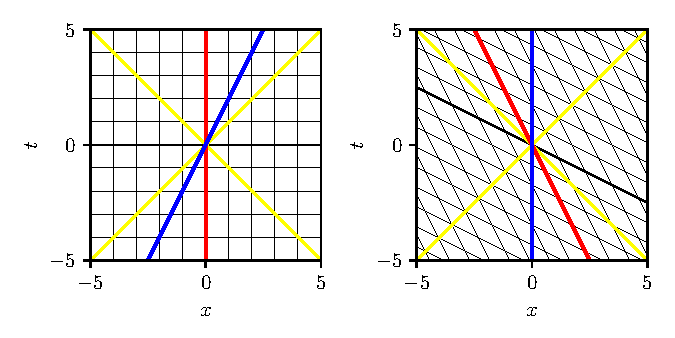
\includegraphics[width=3.2in, height = 1.6in]{images/k1.pdf}
			\caption{A Lorentz Transformation $(k=1)$}
			\label{fig:lorentzk1}
		\end{figure}

		\begin{figure}[h!]
			\centering
			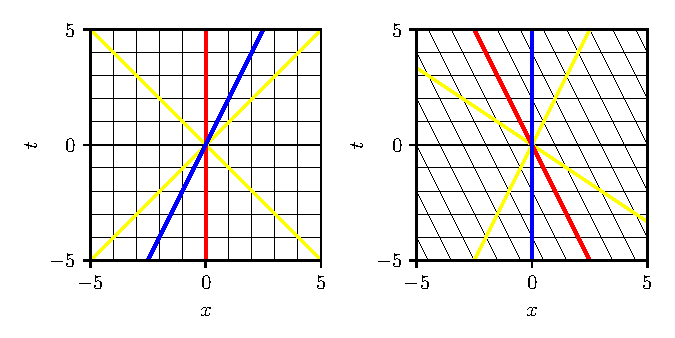
\includegraphics[width=3.2in, height = 1.6in]{images/k0.pdf}
			\caption{A Galilean Transformation $(k=0)$}
			\label{fig:lorentzk0}
		\end{figure}

		\begin{figure}[h!]
			\centering
			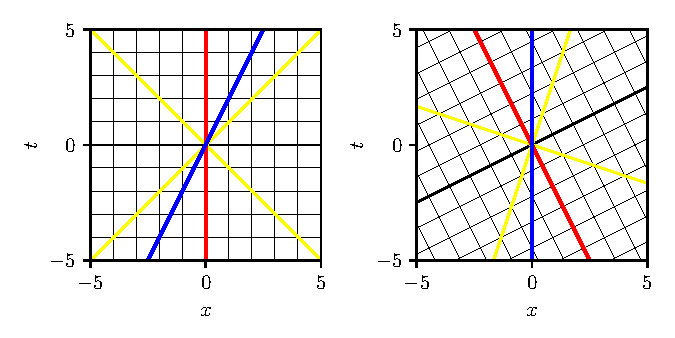
\includegraphics[width=3.2in, height = 1.6in]{images/k-1.pdf}
			\caption{A $k<0$ Lorentz Transformation $(k=-1)$}
			\label{fig:lorentzk-1}
		\end{figure}

	\end{solution_pset}
	\ 
	\newpage
	% ===========================
	% PROBLEM 1.2
	% ===========================
	\stepcounter{subsection}
	\subsection*{
		Problem 1.2
	}
	\begin{problem}
		To get the conditions above, we required closure--- i.e.,
		that the composition of two frame transformations $S\to S'$
		and $S'\to S''$ is also a frame transformation, $S\to S''$.
		You will notice that we only used equality of the diagonal 
		components of the composite transformation to get the equation
		in the problem above. What about the off diagonal components? Explore.
	\end{problem}
	\begin{solution_pset}
		We again refer to \S1.4\cite{juan2026}. For a velocity $w$ with respect from reference frame $S$ 
		to $S''$, transformation obtained has general form
		\begin{equation}
			\label{eq:Mw}
			M\indices{^\mu_\nu}(w)
			=
			\bmqty{
				A(w) & -vA(w) \\[4pt]
				- \dfrac{(A(w)^2-1)}{vA(v)} 
					 & A(w)
			}
		\end{equation}
		As we imposed from the closure condition, we also require
		that the composion of a transformation is also a transformation.
		For velocity $v$ with respect from $S$ to $S'$, and $u$, with respect to 
		$S'$ to $S''$, we have
		\begin{equation}
			\label{eq:Mw-MvMu}
			\tensor{M}{^\mu_\sigma}(w) = \tensor{M}{^\mu_\nu}(u)\tensor{M}{^\nu_\sigma}(v)
		\end{equation}
		Explicitly showing the multiplication, we have
		\[
			\tensor{M}{^\mu_\nu}(w) = 
			\bmqty{
				A(u) & -uA(u) \\[4pt]
				- \dfrac{(A(u)^2-1)}{uA(u)} 
					 & A(u)
			}
			\bmqty{
				A(v) & -vA(v) \\[4pt]
				- \dfrac{(A(v)^2-1)}{vA(v)} 
					 & A(v)
			}
		\]
		Solving that, we have the following monstrous matrix multiplication:
		{
			\begin{equation*}
			\tensor{M}{^\mu_\nu}(w) = 
			\begin{bmatrix}
				A(u)A(v) + \dfrac{uA(u)\bigl(A(v)^2-1\bigr)}{vA(v)} & 
				-(u+v)A(u)A(v) \\[14pt]
				-\dfrac{\bigl(A(u)^2-1\bigr)A(v)}{uA(u)} - \dfrac{A(u)\bigl(A(v)^2-1\bigr)}{vA(v)} & 
				A(u)A(v) + \dfrac{vA(v)\bigl(A(u)^2-1\bigr)}{uA(u)}
			\end{bmatrix}
			\end{equation*}
		}
		We used the equality of diagonal components, i.e, $M\indices{^0_0}$ and $M\indices{^1_1}$, 
		to derive (\ref{eq:A-value}). Now, we are tasked to determine the implications
		of the off-diagonal components, i.e., $M\indices{^0_1}$ and $M\indices{^1_0}$.

		The tricky part here is discerning what it means. The off-diagonal components are not equal, so 
		I can't put a relationship between them, so it took a long time for me to 
		think about what it means. However, I realized that we can again exploit closure.
		That is, components of $M(w)$ must be equal to components of $M(u) M(v)$.
		Also, we already know the value of $A(w)$, which is just (\ref{eq:A-value})
		\[
			A(w) = \frac{1}{\sqrt{1-kw^2}}
		\]
		As a preliminary, we begin with the established result on the lecture, that
		the $M\indices{^1_0}$ reduces to
		\begin{align*}
			-
		   \frac{A(w)^2 - 1}{w A(w)} 
		   &=
		   -
		   \frac{
			   \pqty{\frac{1}{\sqrt{1-kw^2}}}^2 - 1
		   }{w A(w)} \\
		   &=
		   -
		   \frac{
			   {\frac{1}{{1-kw^2}}} - 1
		   }{w A(w)} \\
		   &=
		   -
		   \frac{
			   {\frac{1 - (1-kw^2)}{{1-kw^2}}} 
		   }{w A(w)} \\
		   &=
		   -
		   \frac{
			   {\frac{kw^2)}{{1-kw^2}}} 
		   }{w A(w)} \\
		   &=
		   -
		   \frac{
			   kw^2 A(w)^2
		   }{w A(w)} \\
		   &=
		   -kw A(w)
		\end{align*}
		However, look at $M\indices{^1_0}$, it is just $-w A(w)$.
		Hence, we show the relation between these two components:
		\begin{equation}
			\label{eq:M01-M10 relation}
			M\indices{^0_1} 
			=
			k
			M\indices{^1_0} 
		\end{equation}
		
		With that establish, lets begin working on the problem.
		We start with $M\indices{^1_0}(w)$. By closure, we require that
		\begin{equation}
			\label{eq:M10-equality}
		    w A(w) = (u + v) A(u) A(v)
		\end{equation}
		Likewise, with $M\indices{^0_1}$, we require that
		\begin{equation}
			\label{eq:M01-equality}
			\dfrac{(A(w)^2-1)}{wA(w)} 
			=
			\dfrac{\bigl(A(u)^2-1\bigr)A(v)}{uA(u)} + \dfrac{A(u)\bigl(A(v)^2-1\bigr)}{vA(v)}  
		\end{equation}
		
		We can show that (\ref{eq:M01-equality}) just 
		reduces to (\ref{eq:M10-equality})
		\begin{align*}
			\dfrac{(A(w)^2-1)}{wA(w)} 
			&=
			\dfrac{\bigl(A(u)^2-1\bigr)A(v)}{uA(u)} 
			+
			\dfrac{A(u)\bigl(A(v)^2-1\bigr)}{vA(v)} \\
			\dfrac{kw^2A(w)^2}{wA(w)} 
			&=
			\dfrac{\bigl(ku^2 A(u)^2 \bigr)A(v)}{uA(u)} 
			+
			\dfrac{A(u)\bigl(kv^2 A(v^2)\bigr)}{vA(v)} \\
			kwA(w)
			&=
			kvA(u)A(v)
			+
			kvA(u)A(v)\\
			wA(w)
			&=
			(u+v)
			A(u) A(v)
		\end{align*}

		What we note here is that (\ref{eq:M10-equality}) 
		provides us a consistency condition which determines 
		how $A$ must compose. Now, if we use (\ref{eq:A-value}),
		we find that
		\[ 
			\frac{w}{\sqrt{1 - kw^2}} 
			=
			\frac{u+v}{
				\sqrt{1 - ku^2} 
				\sqrt{1 - kv^2} 
			} 
		\]
		We massage this a bit and look at what we find.
		Consider:
		\begin{align*}
			\frac{w^2}{{1 - kw^2}} 
			&=
			\frac{(u+v)^2}{
				{
					(1 - ku^2)
				} 
				{
					(1 - kv^2)
				} 
			} 
			\\
			w^2
			\pqty{1 - ku^2}
			\pqty{1 - kv^2}
			&=
			(u+v)^2 
			\pqty{1 - kw^2}\\
			w^2
			\pqty{1 - ku^2 - kv^2 + k^2 u^2 v^2}
			&=
			(u+v)^2 
			- kw^2(u+v^2)\\
			w^2
			\pqty{1 - ku^2 - kv^2 + k^2 u^2 v^2}
			+ 
			kw^2(u+v^2)
			&=
			(u+v)^2 \\
			w^2
			\pqty{
				1 - 
				ku^2 - 
				kv^2 + k^2 u^2 v^2 + 
				k(u+v)^2
			}
			&=
			(u+v)^2 \\
			w^2
			\pqty{
				1 - 
				ku^2 - 
				kv^2 + k^2 u^2 v^2 + 
				ku^2 + 2kuv + kv^2
			}
			&=
			(u+v)^2 \\
			w^2
			\pqty{
				1 +
				2kuv + 
				k^2 u^2 v^2 
			}
			&=
			(u+v)^2 \\
			w^2
			(1 + kuv)^2
			&=
			(u+v)^2 \\
			w^2
			&=
			\frac{
				(u+v)^2 
			}{
				(1 + kuv)^2
			} 
		\end{align*}
		Hence, from the equivalence of $M\indices{^1_0}(w) = 
		M\indices{^1_0}(u) 
		M\indices{^1_0}(v) 
		$,
		and the from the scaling factor
		of the components.
		$
		M\indices{^1_0}(w)
		=
		k 
		M\indices{^0_1}(w)
		$,
		out comes the relativistic velocity
		addition law.
		\begin{equation}
			\label{eq:w=u+v}
			\boxed{
				w
				=
				\frac{
					u+v
				}{
					1 + kuv
				}
			}
		\end{equation}

		Note that this relation can be independently
		derived simply from knowing the value of $A$,
		and taking the velocities to be 
		\[
			w = \dv{x}{t} 
		\]
		from $S$ to $S'$,
		and
		\[
			u = \dv{x'}{t'} 
		\]
		from $S''$ to $S'$. You can then do some math
		and still arive with the velocity addition formula.

		However, here we see that the notion velocity addition
		between two moving frames of reference
		is embedded in the components of the transformation itself.
		
	\end{solution_pset}
	\newpage
	% ===========================
	% PROBLEM 1.3
	% ===========================
	\stepcounter{subsection}
	\subsection*{
		Problem 1.3
	}
	\begin{problem}
		Given a basis for a vector space $V$, $\{\vec{e}_i\}, i = 1,\ldots,n$, we considered
		the set of $n$ dual vectors $\{\underline{e}^i\}$ according to the rule
		\begin{equation}
			\label{eq:1.3.1}
			\underline{e}^i[\vec{e}_j] = \tensor{\delta}{^i_j}
		\end{equation}
		\begin{enumerate}[(1)]
			\item Show that this rule is suffient to define the $\underline{e}^i$  as dual
				vectors. That is, we know how each $\underline{e}^i$ acts on all $v\in V$.
			\item Show that $\{\und{e}^i\}$ is a basis for $V^*$.
		\end{enumerate}
	\end{problem}
	\begin{solution_pset}
		% \begin{enumerate}(1)
		    % \item Suffiency of definining it as a dual vector:

				% \begin{proof}
				% \begin{align*}
					% \forall v \in V,\quad \qty{e_\mu} \subset V,\quad \Span{\{e_\mu\}} = V, \qty{e_\mu}&:\\
					% \implies v &= v^\mu e_\mu\\
					% e^\nu[v] &= e^\nu[v^\mu e_\mu]\\
					% e^\nu[v] &= v^\mu e^\nu[e_\mu]\\
					% e^\nu[v] &= v^\mu \delta\indices{^\nu_\mu} \\
					% e^\nu[v] &= v^\nu \\
					% \therefore e^\nu &\in V^*
				% \end{align*}
				% \end{proof}
					
			% \item LI \& spanning
				% \begin{enumerate}

				    % \item LI
						% \begin{proof}
						% \begin{align*}
							% \forall e^\mu \in V^*,\quad e_\nu \in V&\\
							% \forall a_\mu : a_\mu e^\mu &= \und{0}\\
							% \implies a_\mu e^\mu[e_\nu] &= 0\\
							% a_\mu \delta^\mu_\nu &= 0\\
							% \implies\forall a_\nu: a_\nu &= 0\\
							% \implies LI\{e^\mu\} 
						% \end{align*}
						% \end{proof}
						
					% \item Spanning
						% \begin{proof}
						% \begin{align*}
							% \exists e_\mu: e_\mu \in V,\quad& LI \{e_\mu\}, \Span{\{e_\mu\}}=V\\
							% \exists \omega \in V^*&:\\
							% \omega_\mu &= \omega[e_\mu]\\
							% \forall v\in V&:\\
							% \omega[v] &= \omega_\mu e^\mu[v]\\
							% \implies\omega &= \omega_\mu e^\mu\\
							% \therefore \Span{\{e^\mu\}} &= V^* 
						% \end{align*}
						% \end{proof}
				% \end{enumerate}
		% \end{enuerate}
		
		\textit{Note:} I use $\ovr{v}$ instead of $\vec{v}$, it's cleaner looking.

		\begin{enumerate}[(1)]
			\item Suffiency of definining $\und{e}^i$ as a dual vector.

				For the rule $\und{e}^i[\ovr{e}_j]=\delta\indices{^i_j}$ to define $\und{e}^i$ as a dual vector, 
				  we must know how 
				  each $\und{e}^i$ acts on $\ovr{v}$, $\forall \ovr{v}\in V$.

				  By definition (\S 2.6, \cite{juan2026}), a dual vector
				  is a linear map acting on a vector such that, if $\und\omega\in V^*$,
				  $\ovr v\in V$, then
				  \[
					  \omega: V\to \R,\quad \ovr v \mapsto\und\omega[\ovr v]\in \R
				  \]

					\begin{proof}
						Let $\ovr v\in V$. Since $\{\ovr{e}_\mu\}$ is a basis of $V$,
						there exist unique components $v^\mu\in\R$ such that
						\[
							\ovr{v}=v^\mu \ovr{e}_\mu.
						\]
						Then
						\begin{align*}
							\und{e}^\nu[\ovr v]
							&=\und{e}^\nu[v^\mu \ovr{e}_\mu]\\
							&=v^\mu \und{e}^\nu[\ovr{e}_\mu]\\
							&=v^\mu \delta^\nu_\mu\\
							&=v^\nu.
						\end{align*}
						Thus, the action of $\und{e}^\nu$ on every $\ovr v\in V$ is
						completely determined. 
					\end{proof}
			\item For $\qty{\und{e}^i}$ to be a basis, it must be both linearly independent and 
				  spans the entire dual vector space. We prove these two separately.
			
				\begin{enumerate}

					\item Linear Independence.

						If $\qty{\und{e}^i}$ is linearly independent, we note that
						$\forall a_\mu \in \R$, if
						\[
							a_\mu \und{e}^\mu =\und 0,
						\]
						then it implies that $\forall \mu, \mu \in (1,\ldots,n)$,
						\[
							a_\mu = 0.
						\]
						\begin{proof}
							Consider a linear combination such that
							\[
								a_\mu \und e^\mu = \und 0,
							\]
							where $a_\mu\in\mathbb{R}$ are arbitrary.

							Evaluating both sides on $e_\nu\in V$ gives
							\begin{align*}
								a_\mu \und e^\mu[\ovr e_\nu]
								&=\und 0[\ovr e_\nu]\\
								a_\mu\delta^\mu_\nu
								&=0\\
								a_\nu&=0.
							\end{align*}
							Since this holds for every $\nu$, we have
							$a_\mu=0$ for all $\mu$. Hence
							$\{\und e^\mu\}$ is linearly independent.
						\end{proof}
					\item Spanning

						For $\mathrm{span} \qty{\und e^i} = V^*$, it means that
						$\forall \und\omega\in V^*$, $\und\omega$ can be built as a linear combination of the basis vectors,
						i.e.,
						\[
							\und\omega = \omega_\mu \und e^\mu
						\]
						\begin{proof}
							Let $\omega\in V^*$. We define that
							\[
								\omega_\mu=\und \omega[\ovr e_\mu].
							\]
							For any $\ovr v\in V$, we can write
							\[
								\ovr v=v^\mu \ovr e_\mu.
							\]
							Then
							\begin{align*}
								\und\omega[\ovr v]
								&=\und\omega[v^\mu \ovr e_\mu]\\
								&=v^\mu\und\omega[\ovr e_\mu]\\
								&=v^\mu\omega_\mu \\
								&= \omega_\mu v^\mu\\
								&=\omega_\mu \und e^\mu[v].
							\end{align*}

							Since $v$ is arbitrary, we can remove it and
							retain the covector in an operational sense.
							Therefore,
							\[
								\und\omega=\omega_\mu \und e^\mu,
							\]
							so any $\und \omega\in V^*$ is a linear combination
							of $\und e^\mu$. Therefore
							\[
								\mathrm{span}{\{\und e^\mu\}}=V^*.
							\]
							That is, $\und e^\mu$ spans the covector space.
						\end{proof}
				\end{enumerate}

				Hence, $\und e^i$ is a basis for $V^*$.
		\end{enumerate}

	\end{solution_pset}
	\newpage
	% ===========================
	% PROBLEM 1.4
	% ===========================
	\stepcounter{subsection}
	\subsection*{
		Problem 1.4
	}
	\begin{problem}
		Show that if $\{\und{e}^i\}$ is a basis for $V^*$ and 
		$\{\vec{e}_i\}$ is a basis for $V$, then $\qty{\vec{e}_i\otimes \und{e}^j \otimes \und{e}^k}$, $i,j,k = 1,\ldots,n$, is 
		a basis for the space of $(1,2)$ tensors.
	\end{problem}
	\begin{solution_pset}
		
		To show that $\qty{\ovr e_i \otimes \und e^j \otimes \und e^k}$, where $i,j,k=1,\ldots, n$
		is a basis for (1,2) tensors, we must prove that
		it is linearly independent and spans the entire $(1,2)$ tensor space.
		We shall prove these separately.

		\textit{Note:} I will be using abstract index notation here. Also, I will be switching the indices on the basis vectors and covectors to greek because it makes the math easier.

		\begin{enumerate}[(1)]
		    \item Linear Independence.

				% Let the tensor set be 
				% \[
				% 	(T)\indices{^\alpha_{\beta\gamma}}
				% 	=
				% 		\qty{
				% 			\ovr e_\alpha
				% 			\otimes
				% 			\und e^\beta
				% 			\otimes
				% 			\und e^\gamma
				% 		}.
				% \]
				% Here, we denote that $T$ is a tensor for each choice of index $\alpha,\beta,\gamma = 1,\ldots, n$.
				% The parenthesis is there to specify that it is not a component, but rather, a set of tensors. Each choice
				% of index represents members of the basis as the indices $\alpha,\beta,\gamma$, or whatever is specified, varies.

				Let $0\indices{^{a}_{bc}}$ be the zero tensor for the
				$(1,2)$ tensor space, i.e., it maps all covector and vector
				arguments to $0$.

				The set of tensors $
				%	{(T)\indices{^{\alpha}_{\beta\gamma}}}
					\qty{
						\ovr e_\alpha \otimes \und e^\beta \otimes \und e^\gamma
					}
				$ is linearly independent
				if, for all $C\indices{_\alpha^{\beta\gamma}}\in\R$,
				\[
					C\indices{^\alpha_{\beta\gamma}}\ 
					\ovr e_\alpha \otimes \und e^\beta \otimes \und e^\gamma
					=
					0\indices{^{a}_{bc}}
				\]
				implies
				\[
					C\indices{^\alpha_{\beta\gamma}}=0
				\]
				for all $\alpha,\beta,\gamma=1,\ldots,n$.
				% \footnote{I am under the impression here 
				% that \textit{top} and \textit{bottom} index order does not matter, i.e., $C\indices{_\alpha^{\beta\gamma}} = C\indices{^{\beta\gamma}_\alpha}$}.

				\begin{proof}
					% Let
					% \[
					% 	T\indices{^{a}_{bc}}
					% 	=
					% 	{
					% 		\ovr e_\alpha
					% 		\otimes
					% 		\und e^\beta
					% 		\otimes
					% 		\und e^\gamma
					% 	}.
					% \]
					Consider $C\indices{^\alpha_{\beta\gamma}}\in\R$ such that
					\[
						C\indices{^\alpha_{\beta\gamma}}\ 
						% T\indices{^{a}_{bc}}
						\ovr e_\alpha \otimes \und e^\beta \otimes \und e^\gamma
						=
						0\indices{^{a}_{bc}}.
					\]
					Let's feed the tensor a set of basis covectors and vectors,
					$\und e^\lambda,\ovr e_\mu,\ovr e_\nu$.
					Then
					\begin{align*}
						C\indices{^\alpha_{\beta\gamma}}\ 
						% T\indices{^{a}_{bc}}
						\ovr e_\alpha \otimes \und e^\beta \otimes \und e^\gamma
						[
							\und e^\lambda,
							\ovr e_\mu,
							\ovr e_\nu
						]
						&=
						0\indices{^{a}_{bc}}
						[
							\und e^\lambda,
							\ovr e_\mu,
							\ovr e_\nu
						]
						\\
						% C\indices{_\alpha^{\beta\gamma}}
						% \ovr e_\alpha
						% \otimes
						% \und e^\beta
						% \otimes
						% \und e^\gamma
						% [
						% 	\und e^\lambda,
						% 	\ovr e_\mu,
						% 	\ovr e_\nu
						% ]
						% &=0
						% \\
						C\indices{^\alpha_{\beta\gamma}}\ 
						\ovr e_\alpha[\und e^\lambda]
						\und e^\beta[\ovr e_\mu]
						\und e^\gamma[\ovr e_\nu]
						&=0
						\\
						C\indices{^\alpha_{\beta\gamma}}
						\delta\indices{^\lambda_\alpha}
						\delta\indices{^\beta_\mu}
						\delta\indices{^\gamma_\nu}
						&=0
						\\
						C\indices{^\lambda_{\beta\gamma}}
						\delta\indices{^\beta_\mu}
						\delta\indices{^\gamma_\nu}
						&=0
						\\
						C\indices{^\lambda_{\mu\gamma}}
						\delta\indices{^\gamma_\nu}
						&=0
						\\
						C\indices{^\lambda_{\mu\nu}}
						&=0.
					\end{align*}
					Since the indices $\lambda,\mu,\nu$ are arbitrary, we can replace them. Hence,
					\[
						C\indices{^\alpha_{\beta\gamma}}=0
					\]
					for all $\alpha,\beta,\gamma$.
				\end{proof}
				
				
			\item Spanning

				A set of tensors $
					% \qty{T\indices{^{a}_{bc}}}
					\qty{
						\ovr e_\alpha \otimes \und e^\beta \otimes \und e^\gamma
					}
				$ span the tensor space $(1,2)$,
				if an arbitrary tensor $G\indices{^{a}_{bc}}$ can be written as a linear
				combination of the tensor set $G\indices{^\alpha_{\beta\gamma}}\in \R, \forall \alpha,\beta,\gamma = 1,\ldots,n$, i.e.,
				\[
					G\indices{^{a}_{bc}}
					 = 
					 G\indices{^{\alpha}_{\beta\gamma}}\ 
					\ovr e_\alpha \otimes \und e^\beta \otimes \und e^\gamma
				\]

				\begin{proof}
					% Let 
					% \[
					% 	T\indices{^a_{bc}} = \ovr e_\lambda \otimes \und e^\mu \otimes \und e^\nu
					% \]

					We define the following: 

					For an arbitrary tensor $G\indices{^a_{bc}}$,
					we define that the components are given by\footnote{
						I kinda feel like this move is a hack of some sort.
						Feels like a circular argument without really having justification.
						I don't understand why we define it to be like that (other 
						than to define it in terms of the basis itself), but the lecture defined things like
						this multiple times so yeah, just kinda followed it.
					}
					\[
						G\indices{^\alpha_{\beta\gamma}}
						\equiv
						G\indices{^a_{bc}} 
						[
							\und e^\alpha,
							\ovr e_\beta,
							\ovr e_\gamma
						]
					\]
					Thus, let's feed the basis covectors and vectors $
							\und e^\lambda,
							\ovr e_\mu,
							\ovr e_\nu
					$
					\begin{align*}
						G\indices{^a_{bc}} 
						[
							\und e^\lambda,
							\ovr e_\mu,
							\ovr e_\nu
						]
						&=
						G\indices{^\lambda_{\mu\nu}}
						\\
						&=
						G\indices{^\alpha_{\mu\nu}}
						\delta\indices{^\lambda_\alpha}
						\\
						&=
						G\indices{^\alpha_{\beta\nu}}
						\delta\indices{^\lambda_\alpha}
						\delta\indices{^\beta_\mu}
						\\
						&=
						G\indices{^\alpha_{\beta\gamma}}\ 
						\delta\indices{^\lambda_\alpha}
						\delta\indices{^\beta_\mu}
						\delta\indices{^\gamma_\nu}
						\\
						&=
						G\indices{^\alpha_{\beta\gamma}}\ 
						\ovr e_{\alpha}
						[\und e^\lambda]
						\und e^{\beta}
						[\ovr e_\mu]
						\und e^{\gamma}
						[\ovr e_\nu]
						\\
						&=
						G\indices{^\alpha_{\beta\gamma}}
						(
							\ovr e_\alpha \otimes 
							\und e^\beta \otimes 
							\und e^\gamma
						)
						[
							\und e^\lambda,
							\ovr e_\mu,
							\ovr e_\nu
						]
					\end{align*}
					However, the term in the parenthesis is just
					% $T\indices{^a_{bc}}$,
					the tensor set,
					thus
					\begin{align*}
						G\indices{^a_{bc}} 
						[
							\und e^\alpha,
							\ovr e_\beta,
							\ovr e_\gamma
						]
						&=
						G\indices{^\alpha_{\beta\gamma}}\ 
						\ovr e_\alpha \otimes \und e^\beta \otimes \und e^\gamma
						[
							\und e^\lambda,
							\ovr e_\mu,
							\ovr e_\nu
						]
					\end{align*}
					Since the arguments $
						\und e^\lambda,
						\ovr e_\mu,
						\ovr e_\nu
					$ are arbitrary, we can remove them and retain
					the tensor as an operator. Therefore
					\begin{align*}
						G\indices{^a_{bc}} 
						&=
						G\indices{^\alpha_{\beta\gamma}}\ 
						% T\indices{^a_{bc}}
						\ovr e_\alpha \otimes \und e^\beta \otimes \und e^\gamma
						\\
						\implies
						\mathrm{span}\qty{
							\ovr e_\alpha \otimes \und e^\beta \otimes \und e^\gamma
						}
						&=
						\binom{1}{2}
					\end{align*}
					% Since $\lambda, \mu,$ and $\nu$ are arbitrary,
					% we can replace them.
					% \begin{align*}
					% 	G\indices{^a_{bc}} 
					% 	&=
					% 	G\indices{^\alpha_{\beta\gamma}}
					% 	T\indices{^a_{bc}}\\[1em]
					% 	\implies
					% 	\mathrm{span}\qty{T\indices{^a_{bc}}} 
					% 	&=
					% 	\binom{1}{2}
					% \end{align*}
					Thus, the tensors
					\[
						\qty{
							\ovr e_\alpha \otimes \und e^\beta \otimes \und e^\gamma
						}
					\]
					span the $(1,2)$ tensor space.
				\end{proof}
		\end{enumerate}
		Hence, $
		\qty{\ovr e_\alpha \otimes \und e^\beta \otimes \und e^\gamma}
		$ constitute a basis for the $(1,2)$ tensor space.

	\end{solution_pset}
	\newpage
	% ===========================
	% PROBLEM 1.5
	% ===========================
	\stepcounter{subsection}
	\subsection*{
		Problem 1.5
	}
	\begin{problem}
		If $g$ is a $(0,2)$ tensor, then it defines an isomorphism between $V$ and $V^*$,
		i.e., $g:V\to V^*$. Show that the inverse map $g\inv: V^* \to V$, such that 
		$g\inv g = gg\inv = \mathrm{Id}$, is a $(2,0)$ tensor.
	\end{problem}
	\begin{solution_pset}
			\begin{proof}
				A $(2,0)$ tensor is a bilinear map such that, if $\alpha\in(2,0), \omega,\eta\in V^*$
				\[
					\alpha:V^*\times V^*\to \R,\qquad \alpha:\omega,\eta\mapsto \alpha(\omega,\eta).
				\]

				Now we figure out how to massage $g\inv$ to show this property.
				Since $g\in(0,2)$ it accepts two vectors and returns a scalar. 
				However, it can also only accept one,
				and can be defined as a map such that
				\[
					g: V \to V^*.
				\]
				We have the inverse map be 
				\[
					g\inv: V^* \to V.
				\]
				That is, it maps covectors to vectors. Let $\omega,\eta\in V^*$,
				then
				\[
					g\inv(\omega) \in V.
				\]
				Since $\eta$ is a covector, it's a map from $V\to \R$. Hence, we can
				have $\eta$ act on $g\inv(\omega)$,
				\[
					\eta(g\inv(\omega))\in\R.
				\]
				Let us define $g\inv$ to accept two arguments, such that
				\[
					g\inv(\omega,\eta)\equiv
					\eta(g\inv(\omega)) \in \R.
				\]
				Thus, we have shown that $g\inv$ can be a map such that
				\[
					g\inv:V^*\times V^* \to \R.
				\]
				However, this is not enough to include it in the group of $(2,0)$ tensors.

				Since $g\inv:V^* \to V$ is an isomorphism, it implies linearity between covectors, i.e.,
				\[
					g\inv(a \omega_1 + b \omega_2) = a g\inv(\omega_1)+ b g\inv(\omega_2).
				\]
				Let us check bilinearity for two covectors. 

				For $a,b\in\R$, then
				\begin{align*}
					g\inv(a\omega_1 + \omega_2, \eta)
					&=
					\eta\qty(g\inv(a\omega_1 + b\omega_2))\\
					&=
					\eta\qty(g\inv(a\omega_1) + g\inv(b\omega_2))\\
					&=
					a \eta g\inv(\omega_1) + b \eta g\inv(\omega_2)\\
					&=
					a g\inv(\omega_1,\eta) + b  g\inv(\omega_2,\eta).
				\end{align*}
				Similarly,
				\[
					g\inv(\omega,a\eta_1 + b\eta_2) = a g\inv(\omega,\eta_1) + b g\inv(\omega,\eta_2).
				\]
				Thus, $g\inv$ is a bilinear on $V^* \times V^*$, and therefore, a $(2,0)$ tensor.
			\end{proof}

			No longer part of the main proof, but a less rigorous but quicker argument is this:
			Since $g$ is defined to be
			\[
				g = g_{\mu\nu}\p_\mu \otimes \p_\nu.
			\]
			Then its inverse, such that
			\[
				gg\inv = g\inv g = \delta,
			\]
			takes the form
			\[
				g\inv = g^{\mu\nu} \dd{x^\mu}\otimes \dd{x^\nu},
			\]
			where
			\[
				g^{\mu\alpha}g_{\alpha\nu} = \delta\indices{^\mu_\nu}.
			\]
			Hence, $g\inv$ is a $(2,0)$ tensor with components $g^{\mu\nu}$.
	\end{solution_pset}
	\newpage
	% ===========================
	% PROBLEM 1.6
	% ===========================
	\stepcounter{subsection}
	\subsection*{
		Problem 1.6
	}
	\begin{problem}
		Starting from the definition of a tensor as a multilinear map, prove the 
		standard transformation law for $(k,l)$-tensor components under a change of coordinates.
	\end{problem}
	\begin{solution_pset}
		The standard Tensor component transformation law under change of 
		coordinates from $\{x^\sigma\}$ to $\{x'^{\mu}\}$ is \cite{juan2026, Liang2023}
		\begin{equation}
			\label{eq:tensor-transformation-law}
			{T'}\indices{^{{\mu_1}\ldots{\mu_k}}_{{\nu_1}\ldots{\nu_l}}}
			=
			\pdv{x'^{\mu_1}}{x^{\rho_1}} 
			\cdots
			\pdv{x'^{\mu_k}}{x^{\rho_k}} 
			\pdv{x^{\sigma_1}}{x'^{\nu_k}} 
			\cdots
			\pdv{x^{\sigma_l}}{x'^{\nu_l}} 
			\tensor{T}{^{{\rho_1}\ldots{\rho_k}}_{{\sigma_1}\ldots{\sigma_l}}}
		\end{equation}
		We derive it, from the definition alone, as follows:

		\begin{proof}
		The definition of a tensor, as stated from the lecture, is (\S 2.7 \cite{juan2026}):

		A tensor of $(k,l)$ type is a multilinear map 
		from the product of dual and vector spaces to real numbers,
		such that
		\begin{equation}
			\label{eq:tensor-defn}
			T:
			V^*_1 \times 
			V^*_2 \times 
			\cdots
			V^*_k \times
			V_1 \times
			V_2 \times
			\cdots
			V_l
			\to \R
		\end{equation}
		That is, it is a \textit{machine} which accepts covectors ($k$ slots), and vectors ($l$ slots),
		and returns a real number. Multilinearity here means that the tensor is linear in each slot separately.

		Vectors are tensors which accept one covector, and likewise covectors are tensors which accept one vector.
		Hence, we can use basis vectors and basis covectors as a basis for a tensor space. Let $\{x^\mu\}$ 
		be coordinate functions in a manifold $\mcal M$, and 
		$T\in(k,l), \omega_i \in V^*, v^i\in V$
		such that we can define vectors and covectors naturally:
		\[
			v = v^\mu \p_\mu, \qquad \omega = \omega_\mu \dd{x^\mu}
		\]
		Therefore, the basis vectors are $\p_\mu$, and the basis covectors are $\dd{x^\mu}$.

		We define that if we feed the tensor basis vectors and covectors, we recover its components.
		\begin{align*}
			T[\dd{x^{\mu_1}},\cdots,\dd{x^{\mu_k}};\p_{\nu_1},\cdots,\p_{\nu_l}]
			\equiv
			T\indices{^{\mu_1\cdots \mu_k}_{\nu_1\cdots\nu_l}}\ 
		\end{align*}
		We can then expand our way into $k+l$ identity $\delta^{\mu_k}_{\nu_l}$ operations,
		pulling out the basis for each index, separating them, discovering it's an outer product,
		and recovering the tensor as an operational
		definition (see the solution on Problem 1.4.2 which uses this method).

		With all that done,
		we find that a tensor $T\in(k,l)$ defined in a chart $\{x^\mu\}$ 
		has component form, which is the form that we need 
		to define the transformation in general.
		\begin{equation}
			\label{eq:tensor-component-form}
			T = 
			T\indices{^{\mu_1\cdots \mu_k}_{\nu_1\cdots\nu_l}}\ 
			\p_{\mu_1}\otimes \cdots \otimes \p_{\mu_k}
			\otimes
			\dd{x^{\nu_1}}\otimes \cdots \otimes \dd{x^{\nu_1}}
		\end{equation}
		Say we wish to change our coordinates from $\{x^\mu\}$ to $\{y^\sigma\}$.
		Recall how a vector components transform under a change of coordinates:
		\begin{equation}
			\label{eq:vector-transform}
			\pdv{}{y^\sigma} = \pdv{x^\mu}{y^\sigma} \pdv{}{x^\mu} 
		\end{equation}
		Additionally, recall how a covector components transform under a change 
		of coordinates
		\begin{equation}
			\label{eq:covector-transform}
			\dd{y^\sigma} = \pdv{y^\sigma}{x^\mu}\dd{x^\mu} 
		\end{equation}
		Let's rewrite the expression it terms of this change of coordinates.
		We will now explicity write $\p_\mu = \pdv{}{x^\mu}$, since there 
		are multiple coordinates involved.

		We're going from $x^\mu$ to $y^\sigma$, so it's gonna be the 
		inverse of the expressions above.
		\[
			T 
			=
			T\indices{^{\mu_1\cdots \mu_k}_{\nu_1\cdots\nu_l}}\ 
			\pqty{
				\pdv{
					y^{\rho_1}
				}{
					x^{\mu_1}
				}
				\pdv{}{
					y^{\rho_1}
				} 
			}
			\otimes
			\cdots
			\otimes
			\pqty{
				\pdv{
					y^{\rho_k}
				}{
					x^{\mu_k}
				}
				\pdv{}{
					y^{\rho_k}
				} 
			}
			\otimes
			\pqty{
				\pdv{x^{\nu_1}}{y^{\sigma_1}}
				\dd{y^{\sigma_1}} 
			}
			\otimes
			\pqty{
				\pdv{x^{\nu_l}}{y^{\sigma_l}}
				\dd{y^{\sigma_l}} 
			}
		\]
			We can pull out the coordinate transformation coefficients, a.k.a. the Jacobians,
			they're just constants, and the tensor product is a linear operation.
			\begin{equation}
				\label{eq:transform-jacobians}
				T 
				=
					\pdv{
						y^{\rho_1}
					}{
						x^{\mu_1}
					}
					\cdots
					\pdv{
						y^{\rho_k}
					}{
						x^{\mu_k}
					}
					\pdv{x^{\nu_1}}{y^{\sigma_1}}
					\cdots
					\pdv{x^{\nu_l}}{y^{\sigma_l}}
				T\indices{^{\mu_1\cdots \mu_k}_{\nu_1\cdots\nu_l}}\ 
					\pdv{}{y^{\rho_1}} 
				\otimes
				\cdots
				\otimes
					\pdv{}{y^{\rho_k}} 
				\otimes
					\dd{y^{\sigma_1}} 
				\otimes
				\cdots
				\otimes
					\dd{y^{\sigma_l}} 
			\end{equation}
		On the other hand, since $T$ is the same tensor regardless
		of the coordinate system, we can write it in the terms of the $\{y^\sigma\}$
		coordinates directly. We denote the components for this new coordinates to be 
		$T'$
		\begin{equation}
			\label{eq:tensor-component-form-y}
			T = 
			{T'}\indices{^{\rho_1 \cdots \rho_k}_{\sigma_1\cdots\sigma_l}}\ 
			\pdv{}{y^{\rho_1}} \otimes \cdots \otimes \pdv{}{y^{\rho_k}} 
			\otimes
			\dd{y^{\sigma_1}}\otimes \cdots \otimes \dd{y^{\sigma_1}}
		\end{equation}
		Let's compare (\ref{eq:transform-jacobians}) and (\ref{eq:tensor-component-form-y}).
		They are equal, they have the same basis tensors. However, their components are not the same.
		But since both statements are equal, then the components of both forms must also
		be equal, only transformations from one another. Hence, we equate them, and find the following result:
		\begin{equation}
			\label{eq:tensor-component-transform}
			\boxed{
				{T'}\indices{^{\rho_1 \cdots \rho_k}_{\sigma_1\cdots\sigma_l}} 
				=
				\pdv{
					y^{\rho_1}
				}{
					x^{\mu_1}
				}
				\cdots
				\pdv{
					y^{\rho_k}
				}{
					x^{\mu_k}
				}
				\pdv{x^{\nu_1}}{y^{\sigma_1}}
				\cdots
				\pdv{x^{\nu_l}}{y^{\sigma_l}}
				T\indices{^{{\mu_1}\cdots{\mu_k}}_{{\nu_1}\cdots{\nu_l}}} 
			}
		\end{equation}

		Therefore, we have recovered (\ref{eq:tensor-transformation-law}),\footnote{
			With some caveats, it used $x'$ instead of $y$, which isn't really
			a problem since we can just relabel it, and the indices are 
			swapped, but indices are arbitrary, and the swapping is consistent.
			We can just rename it and swap them, but I am too tired, and I neither
			have the drive nor inclination to do so.
			It is equivalent to Eq. (\ref{eq:tensor-transformation-law}). Trust me bro.
		} which is how a component of a $(k,l)$ tensor transforms under a
		coordinate transformation.
		\end{proof}
		


	\end{solution_pset}
	% ===========================
	% PROBLEM 1.7
	% ===========================
	\stepcounter{subsection}
	\subsection*{
		Problem 1.7
	}
	\begin{problem}
		Show that the identity maps
		\begin{equation}
			\label{eq:Id1}
		    \Id_1 : V\to V,\ \Id_1(v)= v, \forall v\in V
		\end{equation}
		\begin{equation}
			\label{eq:Id2}
			\Id_2 : V*\to V*,\ \Id_2(\omega)= \omega, \forall v\in V^*
		\end{equation}
		Can be interpreted as the same $(1,1)$ tensor. What are its components?
		What does this tensor do when it is fed a one-form and a vector? 
		Does this remind you of any other tensorial operation?
	\end{problem}
	\begin{solution_pset}
			We tackle this one first with a functional approach,
			then we do the quicker coordinate-based route.
		\begin{proof}

			A $(1,1)$ identity tensor can be viewed as a map
			\[
				\binom{1}{1}:
				V\to V,\qquad 
				\binom{1}{1}:
				V^* \to V^*
			\]
			or equivalently, as a bilinear map
			\[
				\binom{1}{1}:
				V^*\times V\to \R
			\]

			We start with $\Id_1:V\to V$. 
			For any $v\in V$, then
			\[
				\Id_1[v]= v.
			\]
			We can turn this into a scalar-valued operation
			by feeding the resulting vector to a one-form $\omega\in V^*$:
			\[
				\omega[\Id_1[v]] = \omega[v]
			\]
			As we did in Problem 1.5, we can define this as a bilinear map, a $(1,1)$ tensor
			call it $\delta$\footnote{wow, what a shocker choice of name}, such that
			\[
				\delta(\omega,v) \equiv \omega[v]
			\]

			For $\Id_2:V^*\to V^*$, given $\omega\in V^*$,
			then
			\[
				\Id_2(\omega)= \omega
			\]
			A vector $v$ naturally acts on a one-form by evaluation.
			Alternatively, we could use the fact that the double-dual
			space $V^{**}$ is isomorphic to $V$, $V^{**}\cong V$, so 
			\[
				\Id_2(\omega)[v] \equiv v[\Id_2(\omega)] = \omega(v)
			\]
			Again, we find that
			\[
				\delta(\omega,v)= \omega[v]
			\]
			Both identity maps map $v$ and $\omega$ to the same 
			scalar value. Hence, it is the same $(1,1)$ tensor.
		\end{proof}

		Alternatively, since it a vector and a covector can be represented
		with a vector and covector basis,
		\[
			v = v^\mu \ovr e_\mu,\qquad  \omega = \omega_\nu \und e^\nu
		\]
		Then we have
		\begin{align*}
			\delta(\omega,v) 
			&= 
			\delta[
				v^\mu \ovr e_\mu,
				\omega_\nu \und e^\nu
			]\\
			&=
			v^\mu \omega_\nu \delta[\ovr e_\mu, \und e^\nu]\\
			&=
			v^\mu \omega_\nu \delta\indices{^\mu_\nu}\\
			&=
			v^\mu \omega_\nu
		\end{align*}
		That is, it is just the Euclidean tensor/metric,
		or the Kronecker delta, or whatever other name it has.

		Thus, its components are 
		\[
			\delta\indices{^\mu_\nu} = 
			\begin{cases}
			    1,\quad\mu=\nu\\
				0,\quad\mu\neq\nu
			\end{cases}
		\]
		Since it is a $(1,1)$ tensor, and matrices are isomorphic to $(1,1)$ tensors,
		it can be represented as a matrix
		\[
			\delta\indices{^\mu_\nu}
			=
			\bmqty{
				1 & 0 \\
				0 & 1
			} 
		\]
		When fed a one-form and a vector, it simply evaluates the
		one-form on the vector
		\[
			\delta(\omega,v) = \omega(v)
		\]

		Otherwise known as a contraction operation, where
		we contract the indices upstairs and downstairs.
		\[
			\delta\indices{^\mu_\nu} \omega_\mu v^\nu = \omega_\nu v^\nu = \omega(v)
		\]
		So the identity $(1,1)$ tensor is just the Euclidean metric, or 
		the Kronecker delta, or the identity under contraction operator.
		Among other names.
	\end{solution_pset}
